\chapter{Descriptive Statistics}

% \subsection{ Dữ liệu CPU}
% Code:
% \begin{figure}[p]
%  \centering
%  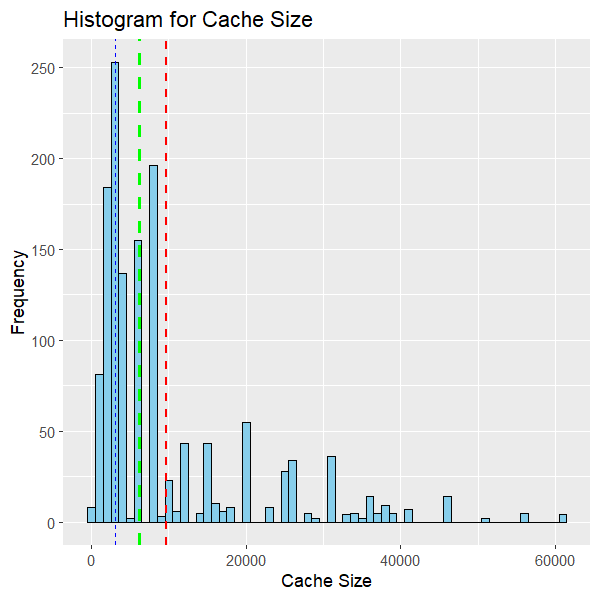
\includegraphics[width=0.33\linewidth]{CPU_histo_Cache.png}\hfill
%  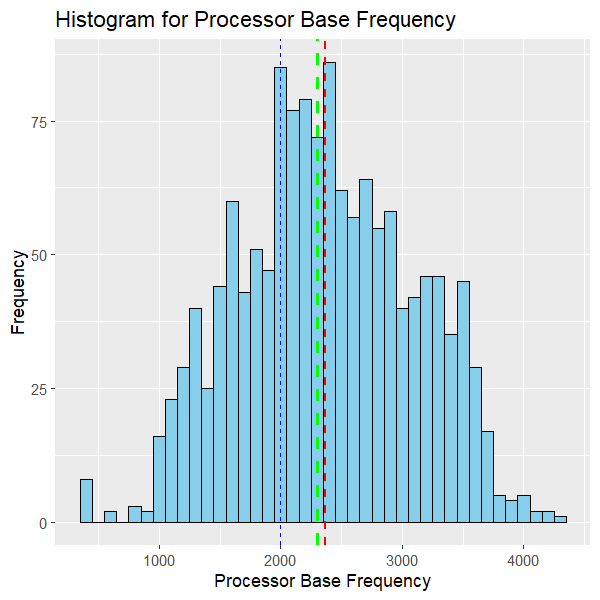
\includegraphics[width=0.33\linewidth]{CPU_histo_Freq.png}\hfill
%  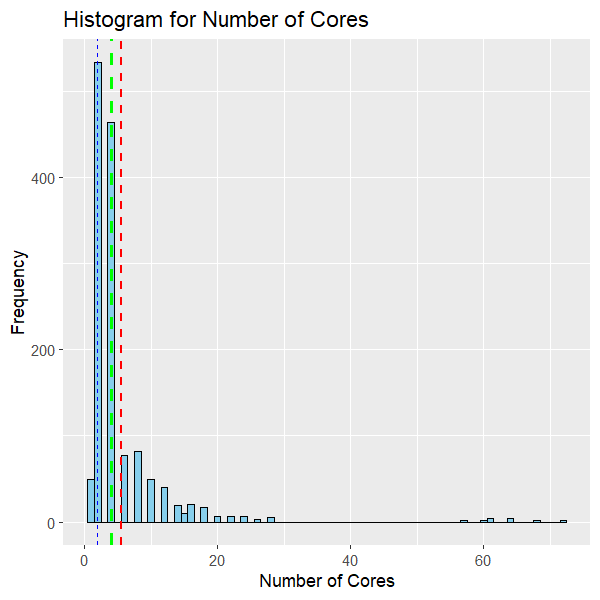
\includegraphics[width=0.33\linewidth]{CPU_histo_Core.png}
%  \\[\smallskipamount]
%  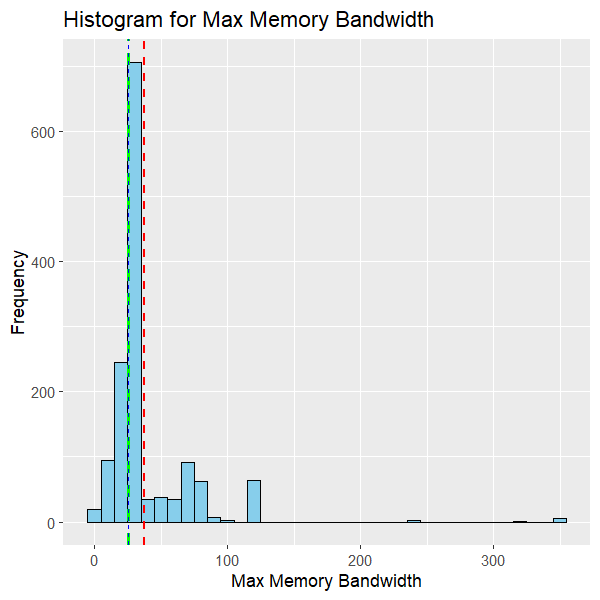
\includegraphics[width=0.33\linewidth]{CPU_histo_MMB.png}\hfill
%  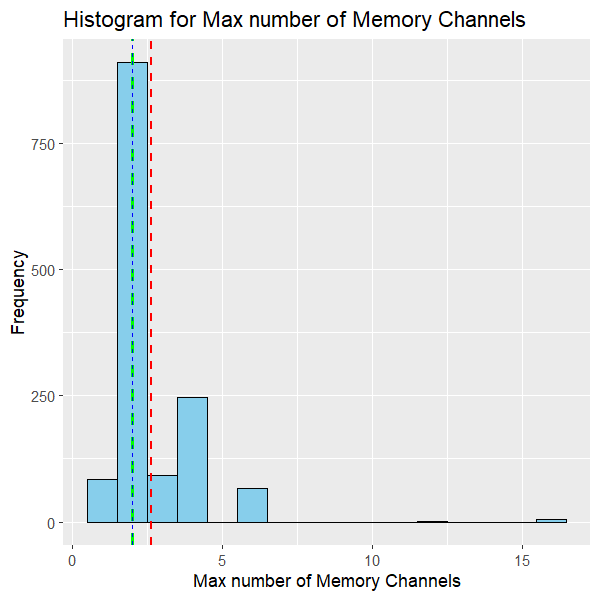
\includegraphics[width=0.33\linewidth]{CPU_histo_MNMC.png}\hfill
%  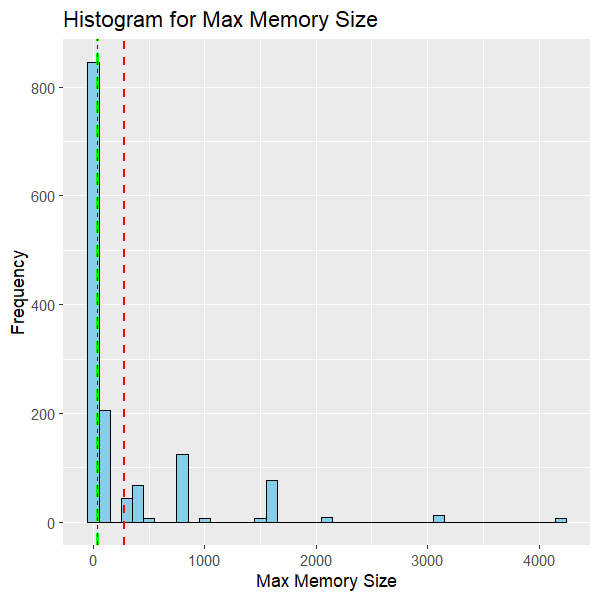
\includegraphics[width=0.33\linewidth]{CPU_histo_MMS.png}
%  \\[\smallskipamount]
%  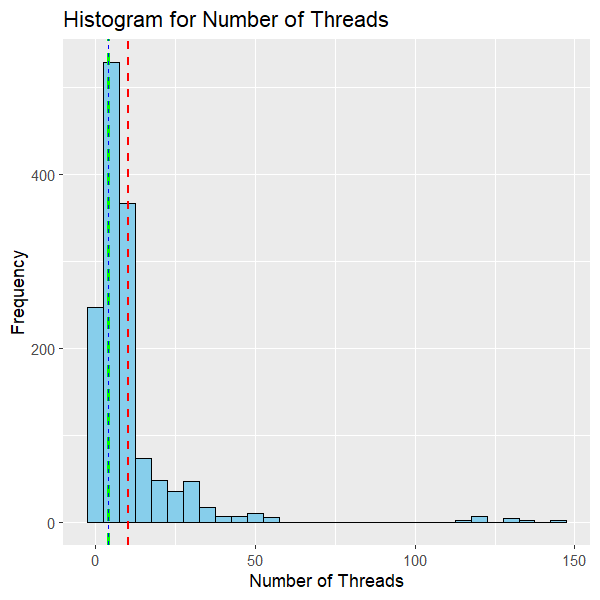
\includegraphics[width=0.33\linewidth]{CPU_histo_Thread.png}\hfill
%  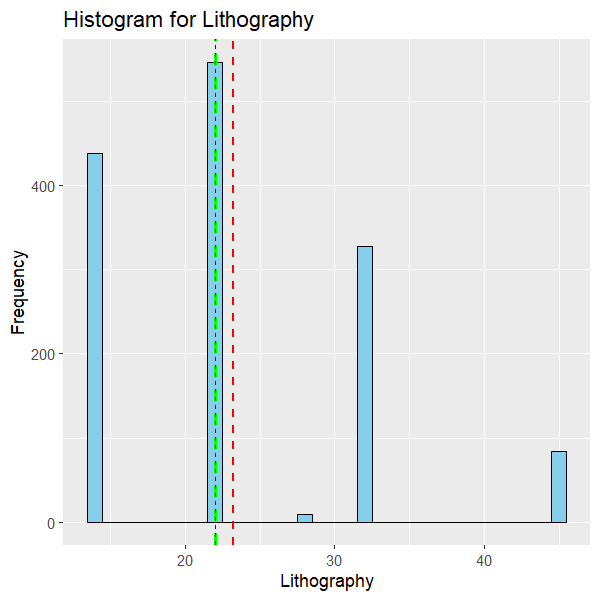
\includegraphics[width=0.33\linewidth]{CPU_histo_Litho.png}\hfill
%  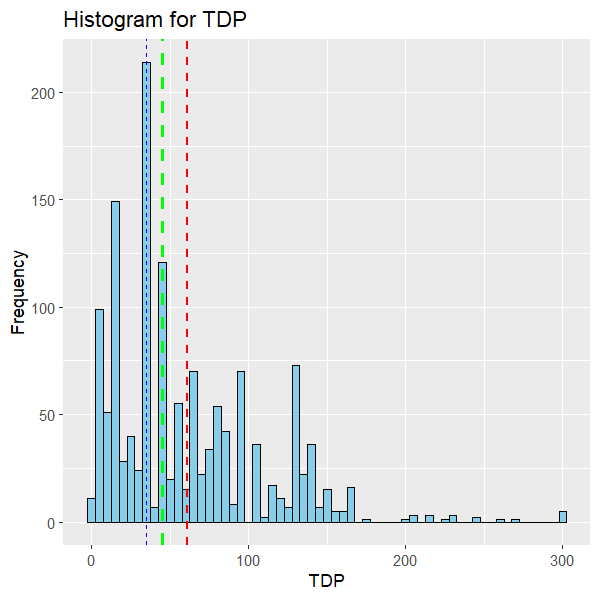
\includegraphics[width=0.33\linewidth]{CPU_histo_TDP.png}
%  \vspace{10pt}
%  \caption{Biểu đồ tần số của các biến trong mẫu từ Intel\_CPUs.csv}
%  \label{fig:Na_GPU}
% \end{figure}
% \begin{lstlisting}[language=R]
% Litho_year <- Intel_clean %>% 
%   group_by(Launch_Year) %>%
%   summarize(mean_litho = mean(Lithography),
%             median_litho = median(Lithography),
%     .groups = "drop"
%   )
% options(repr.plot.width = 15, repr.plot.height =8)
% ggplot(Litho_year, aes(x = Launch_Year)) +
%   geom_line(aes(y = mean_litho, color = "Mean")) +
%   geom_line(aes(y = median_litho, color = "Median")) +
%   scale_color_manual(values = c("Mean" = "blue", "Median" = "red")) +
%   labs(x = "Year", y = "Lithography", title = "Mean and Median Lithography by Year") +
%   scale_x_continuous(breaks = seq(min(Litho_year$Launch_Year), max(Litho_year$Launch_Year),
%   by = 1)) +
%   theme_minimal()
% \end{lstlisting}
% Kết quả:

% \begin{figure}[h]
%  \centering
%  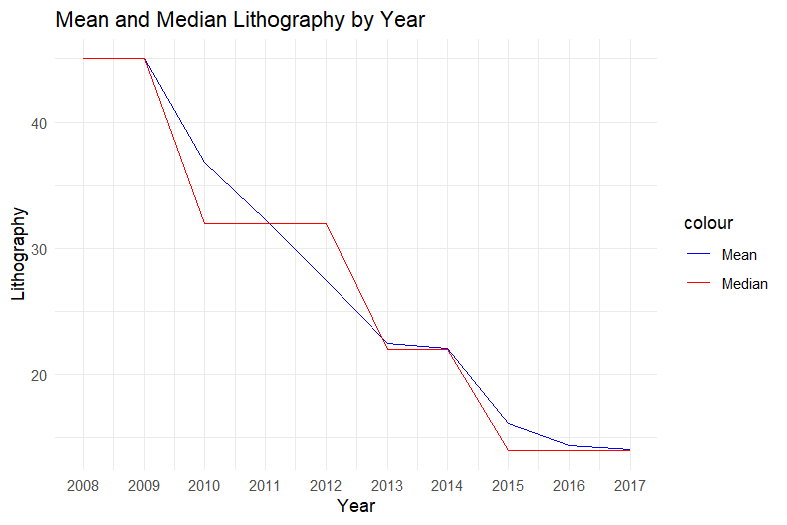
\includegraphics[width=1\linewidth]{img/Litho_Year.png}
%  \vspace{1pt} % adjust the space as needed
%  \caption{Enter Caption}
%  \label{fig:enter-label}
% \end{figure}

% \newpage
% Code:
% \begin{lstlisting}[language=R]
% options(repr.plot.width = 15, repr.plot.height =8) 
% ggplot(data = Intel_clean, aes(y = Status, x = Launch_Year, fill = Status)) +
%   geom_boxplot() +
%   labs(x = "Status", y = "Launch Date",title = "Boxplot of Status over Year") +
%   scale_x_continuous(breaks = seq(min(Litho_year$Launch_Year), max(Litho_year$Launch_Year), by = 1))
% \end{lstlisting}
% Kết quả:

% \begin{figure}[h]
%  \centering
%  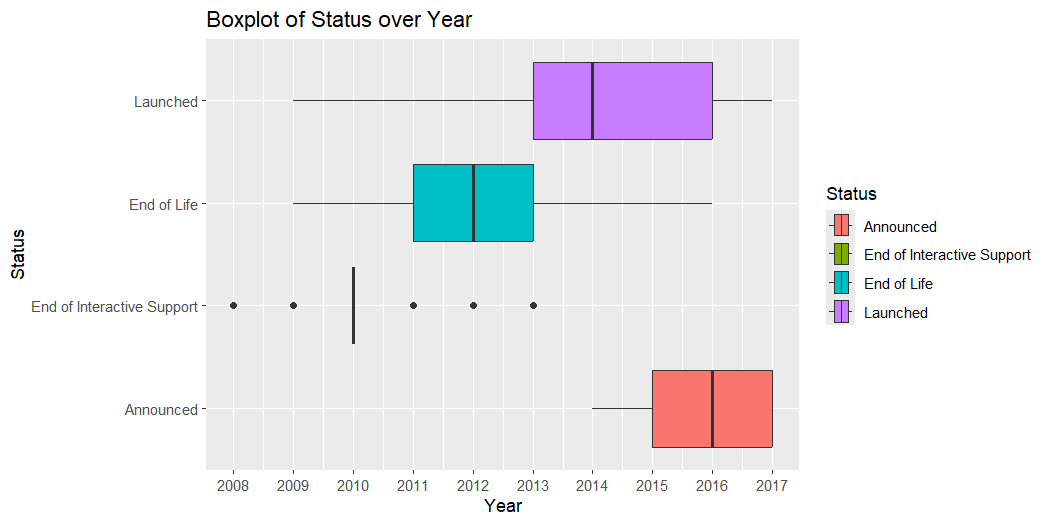
\includegraphics[width=1\linewidth]{img/Status_Year.png}
%  \vspace{1pt}
%  \caption{Enter Caption}
%  \label{fig:enter-label}
% \end{figure}

% Nhận xét:

% \newpage
% Code:
% \begin{lstlisting}[language=R]
% options(repr.plot.width = 15, repr.plot.height =8) 
% ggplot(data = Intel_clean, aes(y = Vertical_Segment, x = Launch_Year, fill = Vertical_Segment)) +
%   geom_boxplot() +
%   labs(x = "Year", y = "Vertical Segment",title = "Boxplot of Vertical Segment over Year") +
%   scale_x_continuous(breaks = seq(min(Litho_year$Launch_Year), max(Litho_year$Launch_Year), by = 1))
% \end{lstlisting}
% Kết quả:

% \begin{figure}[h]
%  \centering
%  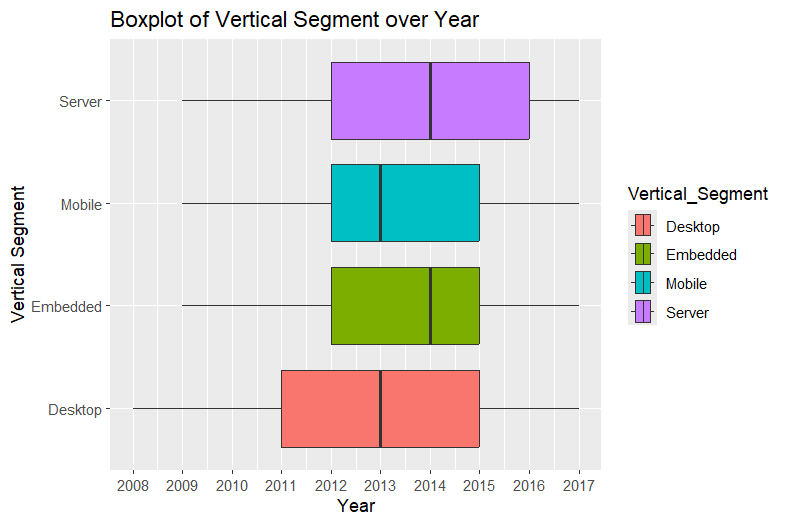
\includegraphics[width=1\linewidth]{img/VSegment_Year.png}
%  \vspace{1pt}
%  \caption{Enter Caption}
%  \label{fig:enter-label}
% \end{figure}

% Nhận xét:

% \newpage
% Code:
% \begin{lstlisting}[language=R]
% options(repr.plot.width = 15, repr.plot.height =8) 
% ggplot(data = Intel_clean, aes(y = Instruction_Set, x = Launch_Year, fill = Instruction_Set)) +
%   geom_violin() +
%   labs(x = "Launch Date", y = "Instruction set",title = "Violinplot of Instruction set over Year") +
%   scale_x_continuous(breaks = seq(min(Litho_year$Launch_Year), max(Litho_year$Launch_Year), by = 1))
% \end{lstlisting}
% Kết quả:

% \begin{figure}[h]
%  \centering
%  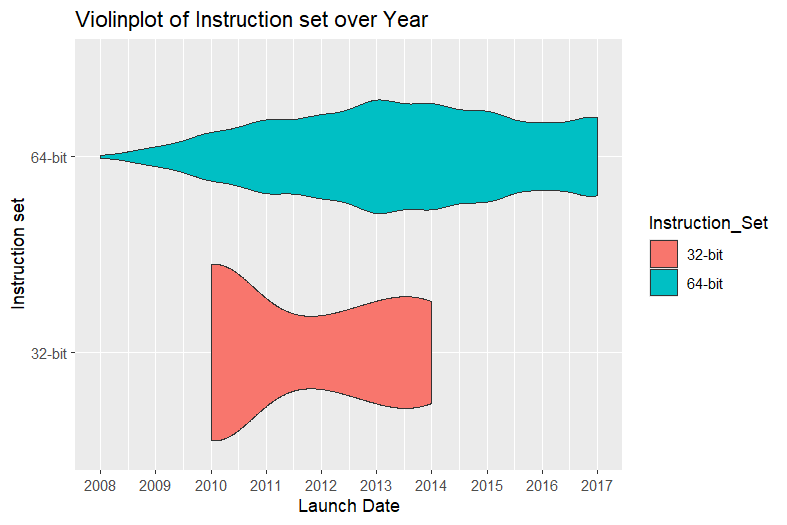
\includegraphics[width=1\linewidth]{img/6432bit_year.png}
%  \vspace{1pt}
%  \caption{Enter Caption}
%  \label{fig:enter-label}
% \end{figure}

% Nhận xét:

% \newpage
% Code:
% \begin{lstlisting}[language=R]
% options(repr.plot.width = 15, repr.plot.height =8) 
% ggplot(data = Intel_clean, aes(y = Instruction_Set, x = Launch_Year, fill = Instruction_Set)) +
%   geom_violin() +
%   labs(x = "Launch Date", y = "Instruction set",title = "Violinplot of Instruction set over Year") +
%   scale_x_continuous(breaks = seq(min(Litho_year$Launch_Year), max(Litho_year$Launch_Year), by = 1))
% \end{lstlisting}
% Kết quả:

% \begin{figure}[h]
%  \centering
%  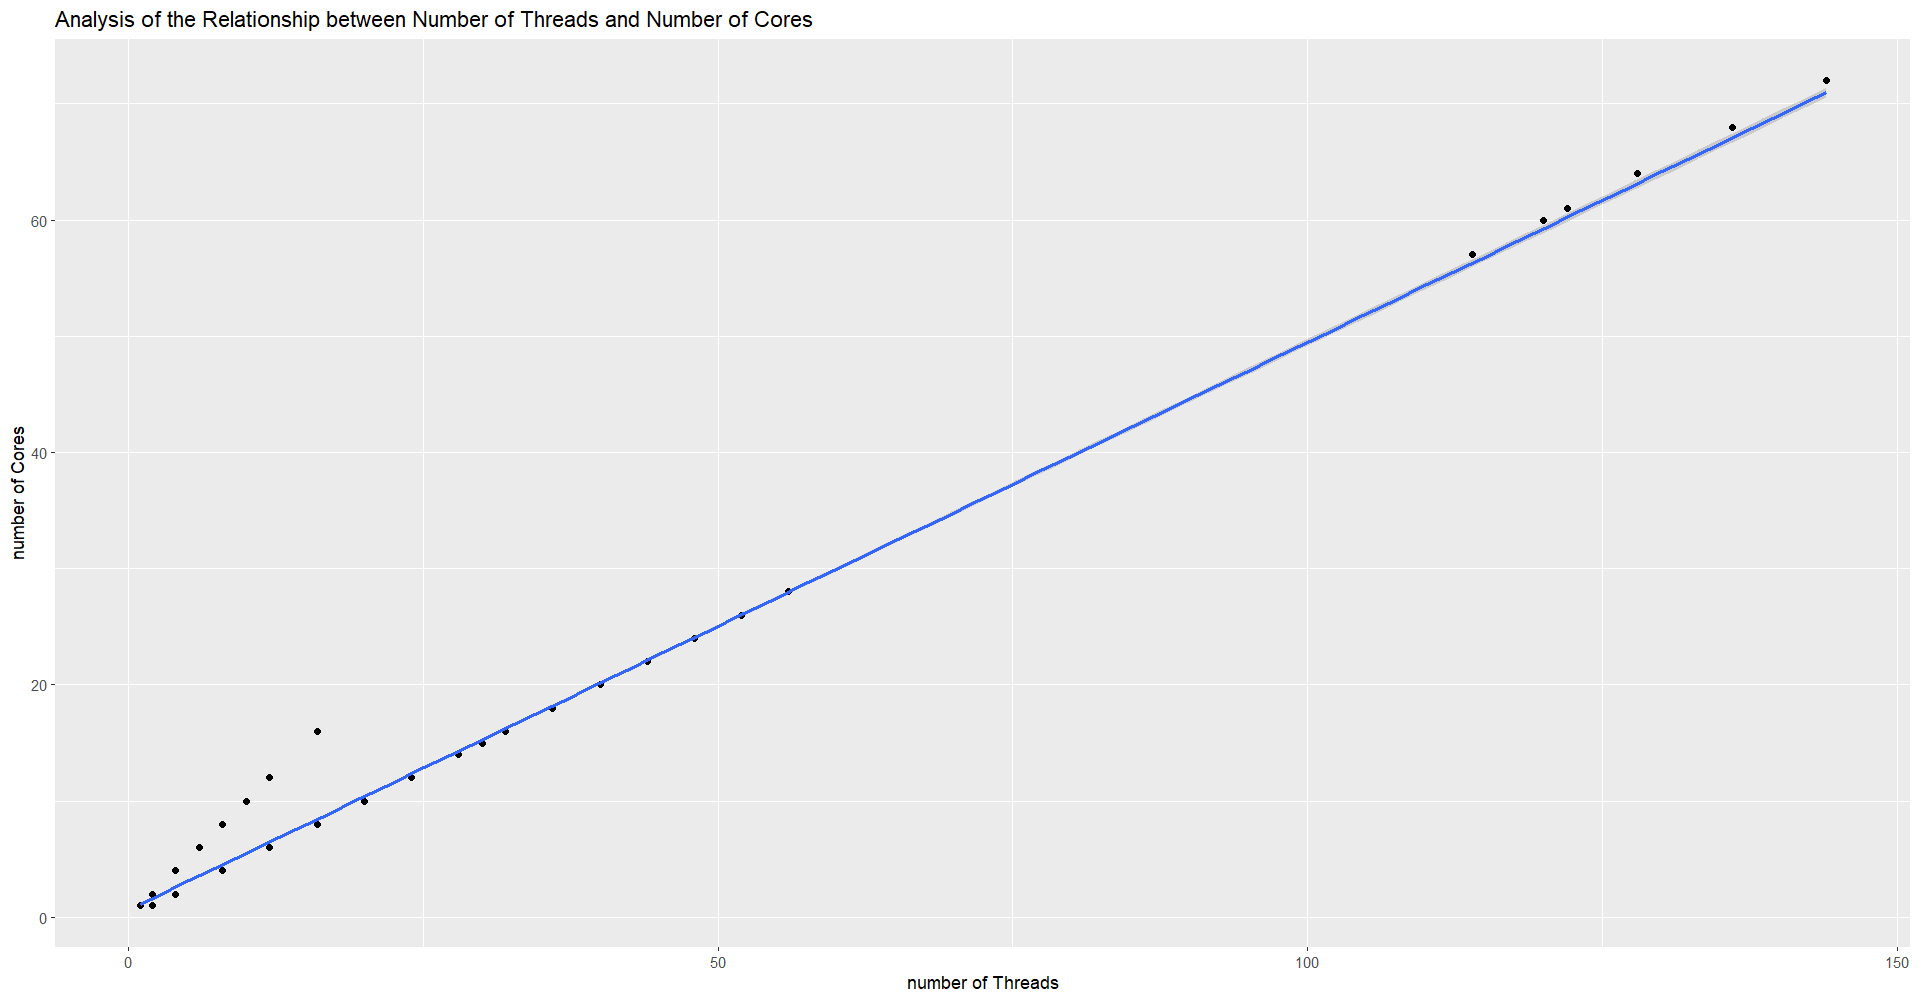
\includegraphics[width=1\linewidth]{img/CPU_ThreadCore.png}
%  \vspace{1pt}
%  \caption{Enter Caption}
%  \label{fig:enter-label}
% \end{figure}

% Nhận xét:

% \newpage
% Kết quả:

% \begin{figure}[h]
%  \centering
%  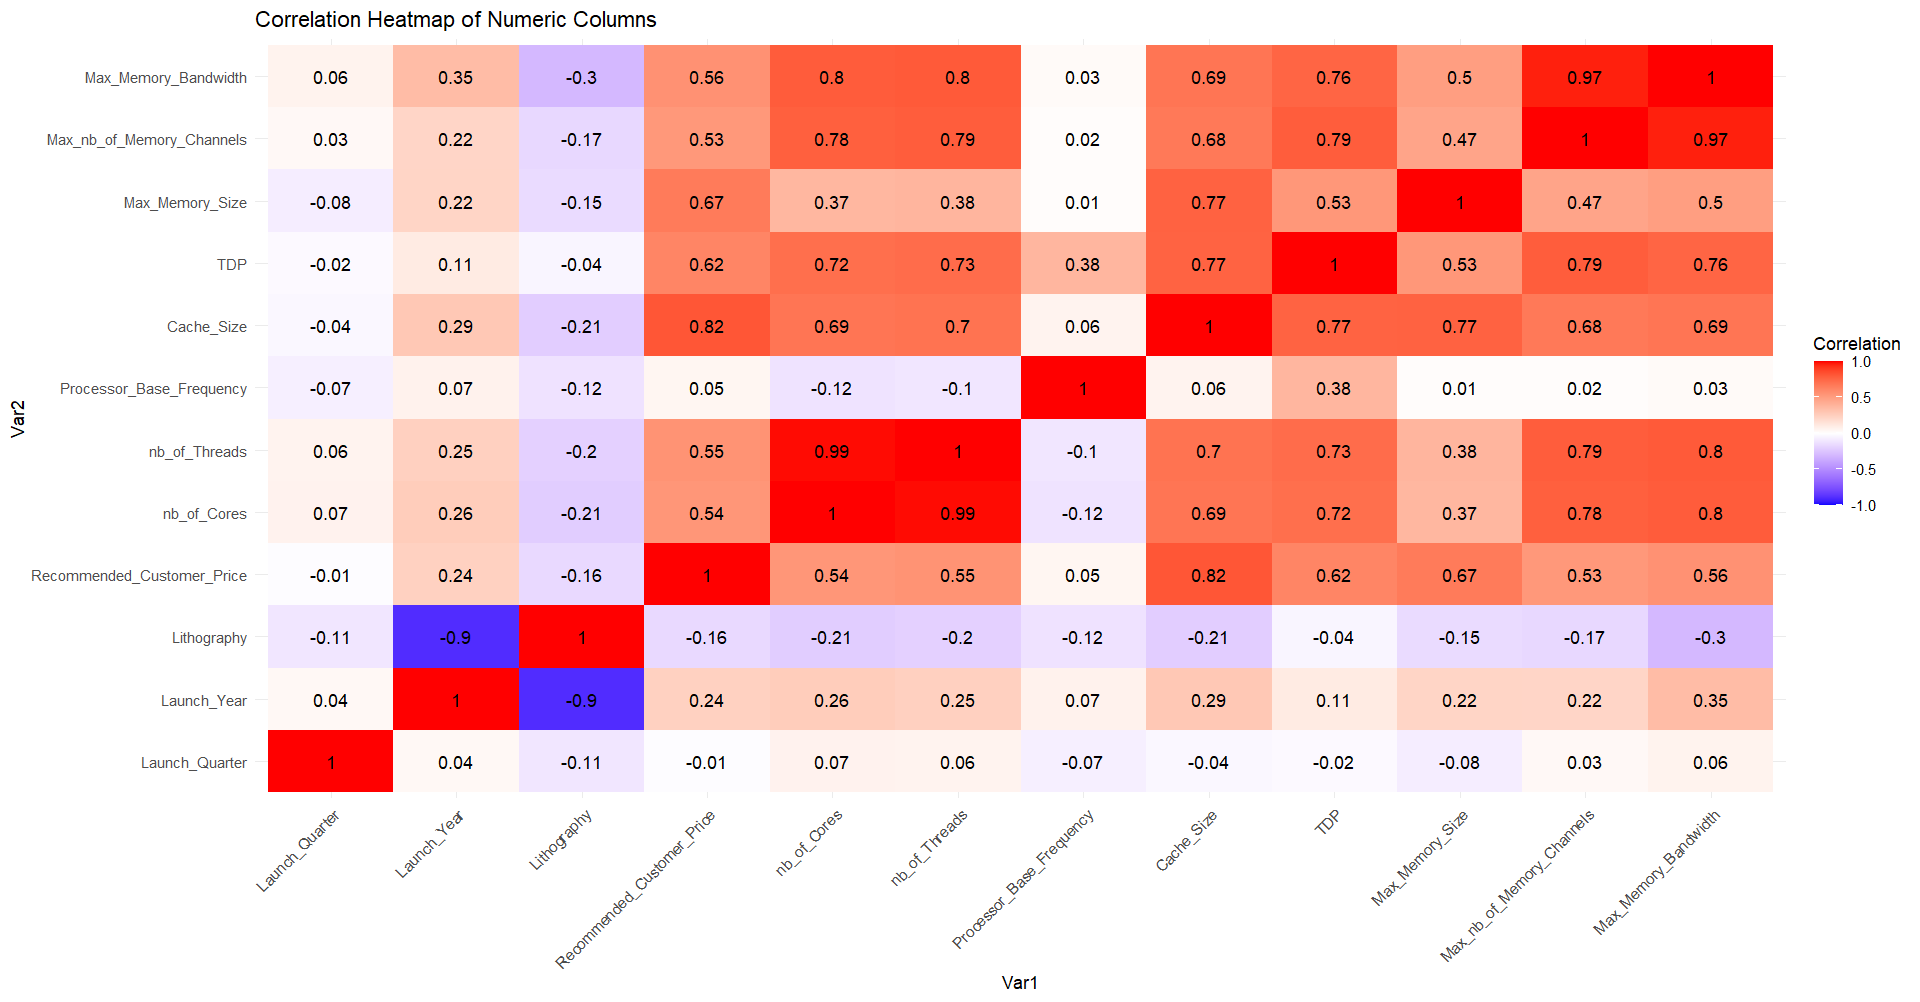
\includegraphics[width=1\linewidth]{img/CPU_cor.png}
%  \vspace{1pt}
%  \caption{Enter Caption}
%  \label{fig:enter-label}
% \end{figure}

% Nhận xét:


% \newpage
% \subsection{ Dữ liệu GPU}
% Code:
% \begin{lstlisting}[language=R]
% freq <- table(clean_GPUs$Manufacturer, clean_GPUs$Release_Year)
% total_count <- colSums(freq)
% percentage <- prop.table(freq, margin = 2) * 100

% barplot(freq,
%         legend.text = TRUE,
%         main = "Counts of Each Year",
%         xlab = "Year",
%         ylab = "Count",
%         col = c("skyblue", "salmon", "lightgreen", "yellow"),
%         border = "black")
% \end{lstlisting}
% Kết quả:

% \begin{figure}[h]
%  \centering
%  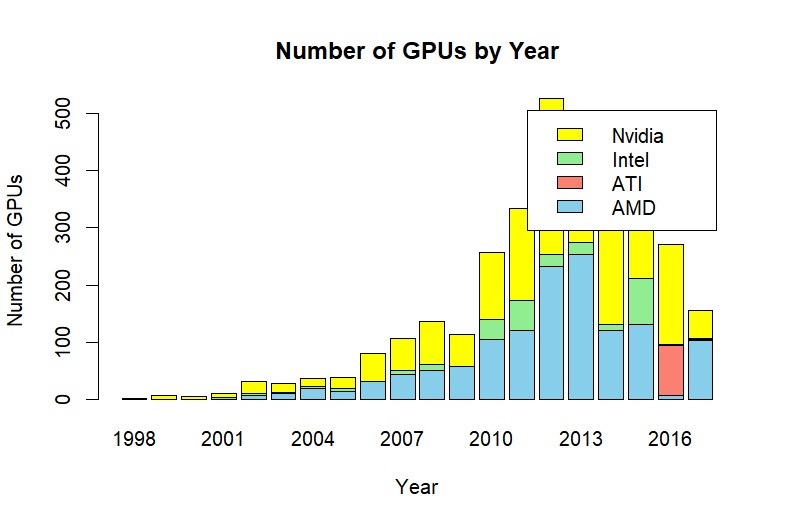
\includegraphics[width=1\linewidth]{img/Market_Year.png}
%  \vspace{1pt}
%  \caption{Enter Caption}
%  \label{fig:enter-label}
% \end{figure}

% Nhận xét:

% \newpage
% Code:
% \begin{lstlisting}[language=R]
% barplot(percentage,
%         legend.text = TRUE,
%         main = "Market Share Percentage by Year",
%         xlab = "Year",
%         ylab = "Percentage",
%         col = c("skyblue", "salmon", "lightgreen", "yellow"),
%         border = "black")
% \end{lstlisting}
% Kết quả:

% \begin{figure}[h]
%  \centering
%  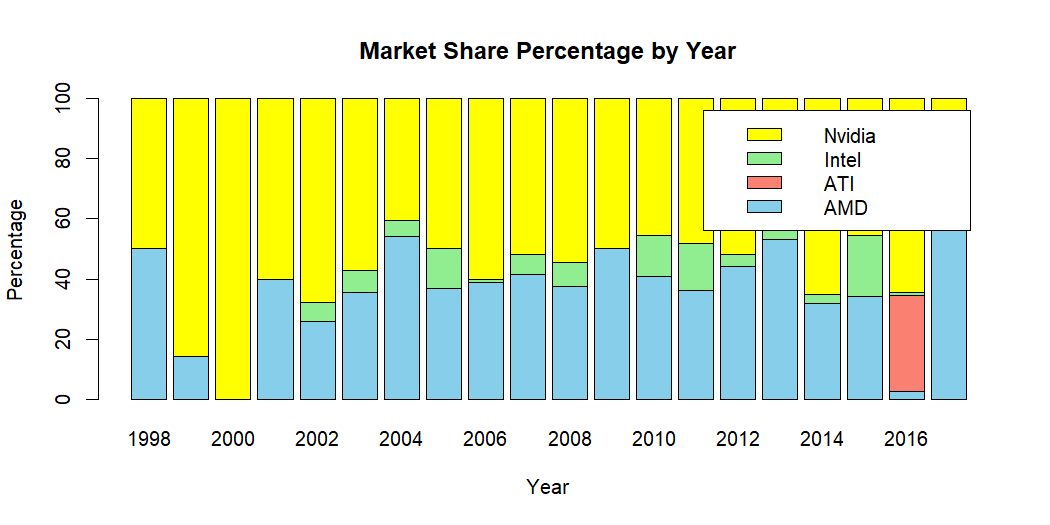
\includegraphics[width=1\linewidth]{img/Market_Percent_Year.png}
%  \vspace{1pt}
%  \caption{Enter Caption}
%  \label{fig:enter-label}
% \end{figure}

% Nhận xét:

% \newpage
% Code:
% \begin{lstlisting}[language=R]
% scatter_plot <- ggplot(clean_GPUs, aes(x = Release_Year + Release_Month/12, y = Memory, color = Manufacturer)) +
%   geom_point() +
%   scale_color_manual(values = c("skyblue", "salmon", "lightgreen", "yellow")) +
%   labs(x = "Year", y = "GPU Memory", title = "Scatter Plot of GPU Memory vs Year") +
%   theme_minimal()
% print(scatter_plot)
% \end{lstlisting}
% Kết quả:

% \begin{figure}[h]
%  \centering
%  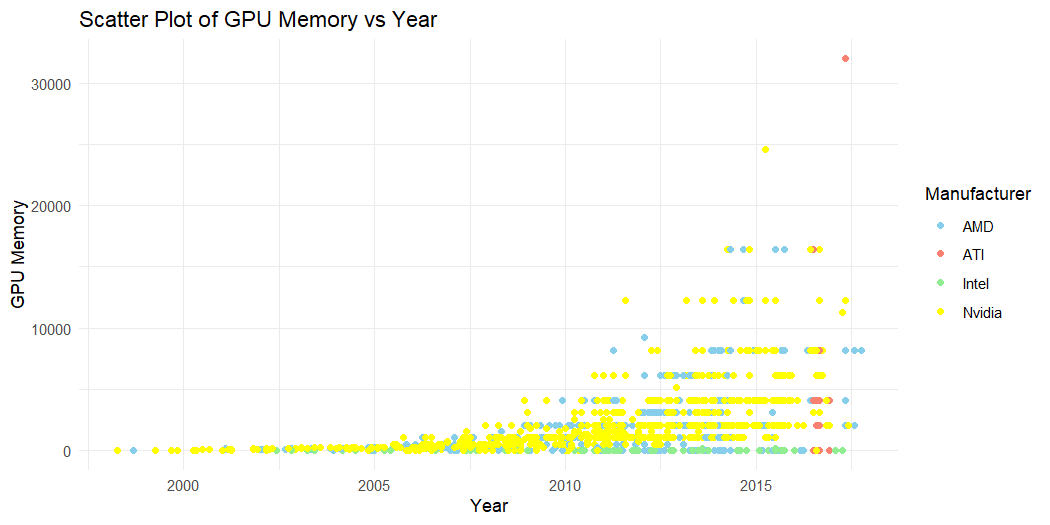
\includegraphics[width=1\linewidth]{img/GPU_Memo_Year.png}
%  \vspace{1pt}
%  \caption{Enter Caption}
%  \label{fig:enter-label}
% \end{figure}

% Nhận xét:

% \newpage
% Code:
% \begin{lstlisting}[language=R]
% memory_summary <- clean_GPUs %>%
%   group_by(Release_Year) %>%
%   summarise(mean_memory = mean(Memory),
%             median_memory = median(Memory))

% line_plot <- ggplot(memory_summary, aes(x = Release_Year)) +
%   geom_line(aes(y = mean_memory, color = "Mean")) +
%   geom_line(aes(y = median_memory, color = "Median")) +
%   scale_color_manual(values = c("Mean" = "blue", "Median" = "red")) +
%   labs(x = "Year", y = "Memory", title = "Mean and Median Memory by Year") +
%   theme_minimal()
% print(line_plot)
% \end{lstlisting}
% Kết quả:

% \begin{figure}[h]
%  \centering
%  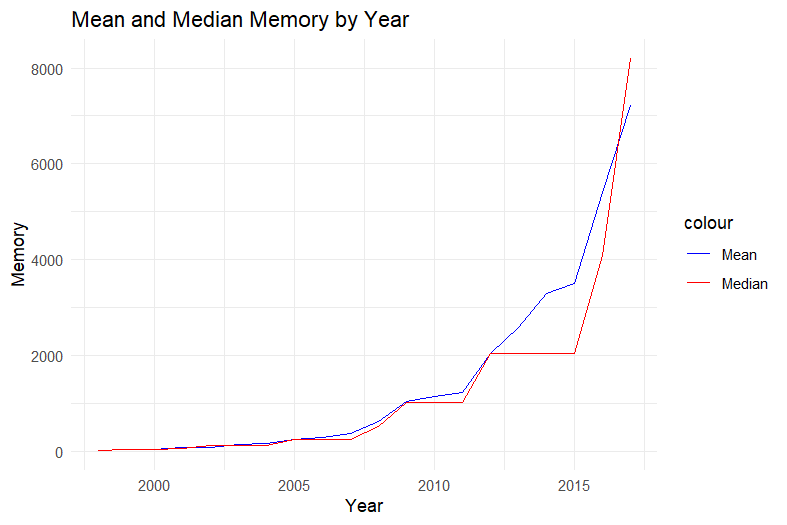
\includegraphics[width=1\linewidth]{img/MeaMedMem_Year.png}
%  \vspace{1pt}
%  \caption{Enter Caption}
%  \label{fig:enter-label}
% \end{figure}

% Code:
% \begin{lstlisting}[language=R]
% moore_law <- data.frame(
%   Release_Year = seq(min(memory_summary$Release_Year), max(memory_summary$Release_Year), 1),
%   Memory = 2^(0.5 * (seq(min(memory_summary$Release_Year), max(memory_summary$Release_Year), 1) - min(memory_summary$Release_Year - 8)))
% )

% memory_summary$log_mean_memory <- log(memory_summary$mean_memory)
% memory_summary$log_median_memory <- log(memory_summary$median_memory)

% line_plot <- ggplot(memory_summary, aes(x = Release_Year)) +
%   geom_line(aes(y = log_mean_memory, color = "Logarithm of Mean"), size = 1) +
%   geom_line(aes(y = log_median_memory, color = "Logarithm of Median"), size = 1) +
%   geom_line(data = moore_law, aes(y = log(Memory), color = "Moore's Law"), size = 1, linetype = "dashed") +
%   scale_color_manual(values = c("Logarithm of Mean" = "blue", "Logarithm of Median" = "red", "Moore's Law" = "green4")) +
%   labs(x = "Year", y = "Logarithm of Memory", title = "Logarithm of Mean and Median Memory by Year") +
%   theme_minimal()

% print(line_plot)
% \end{lstlisting}
% Kết quả:

% \begin{figure}[h]
%  \centering
%  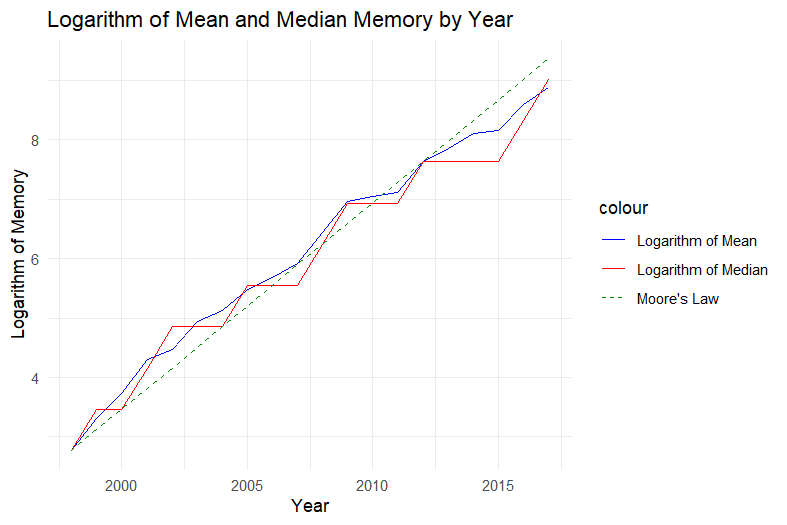
\includegraphics[width=1\linewidth]{img/LogMeaMedMem_Year.png}
%  \vspace{1pt}
%  \caption{Enter Caption}
%  \label{fig:enter-label}
% \end{figure}

% Nhận xét:

% \newpage
% Kết quả:

% \begin{figure}[h]
%  \centering
%  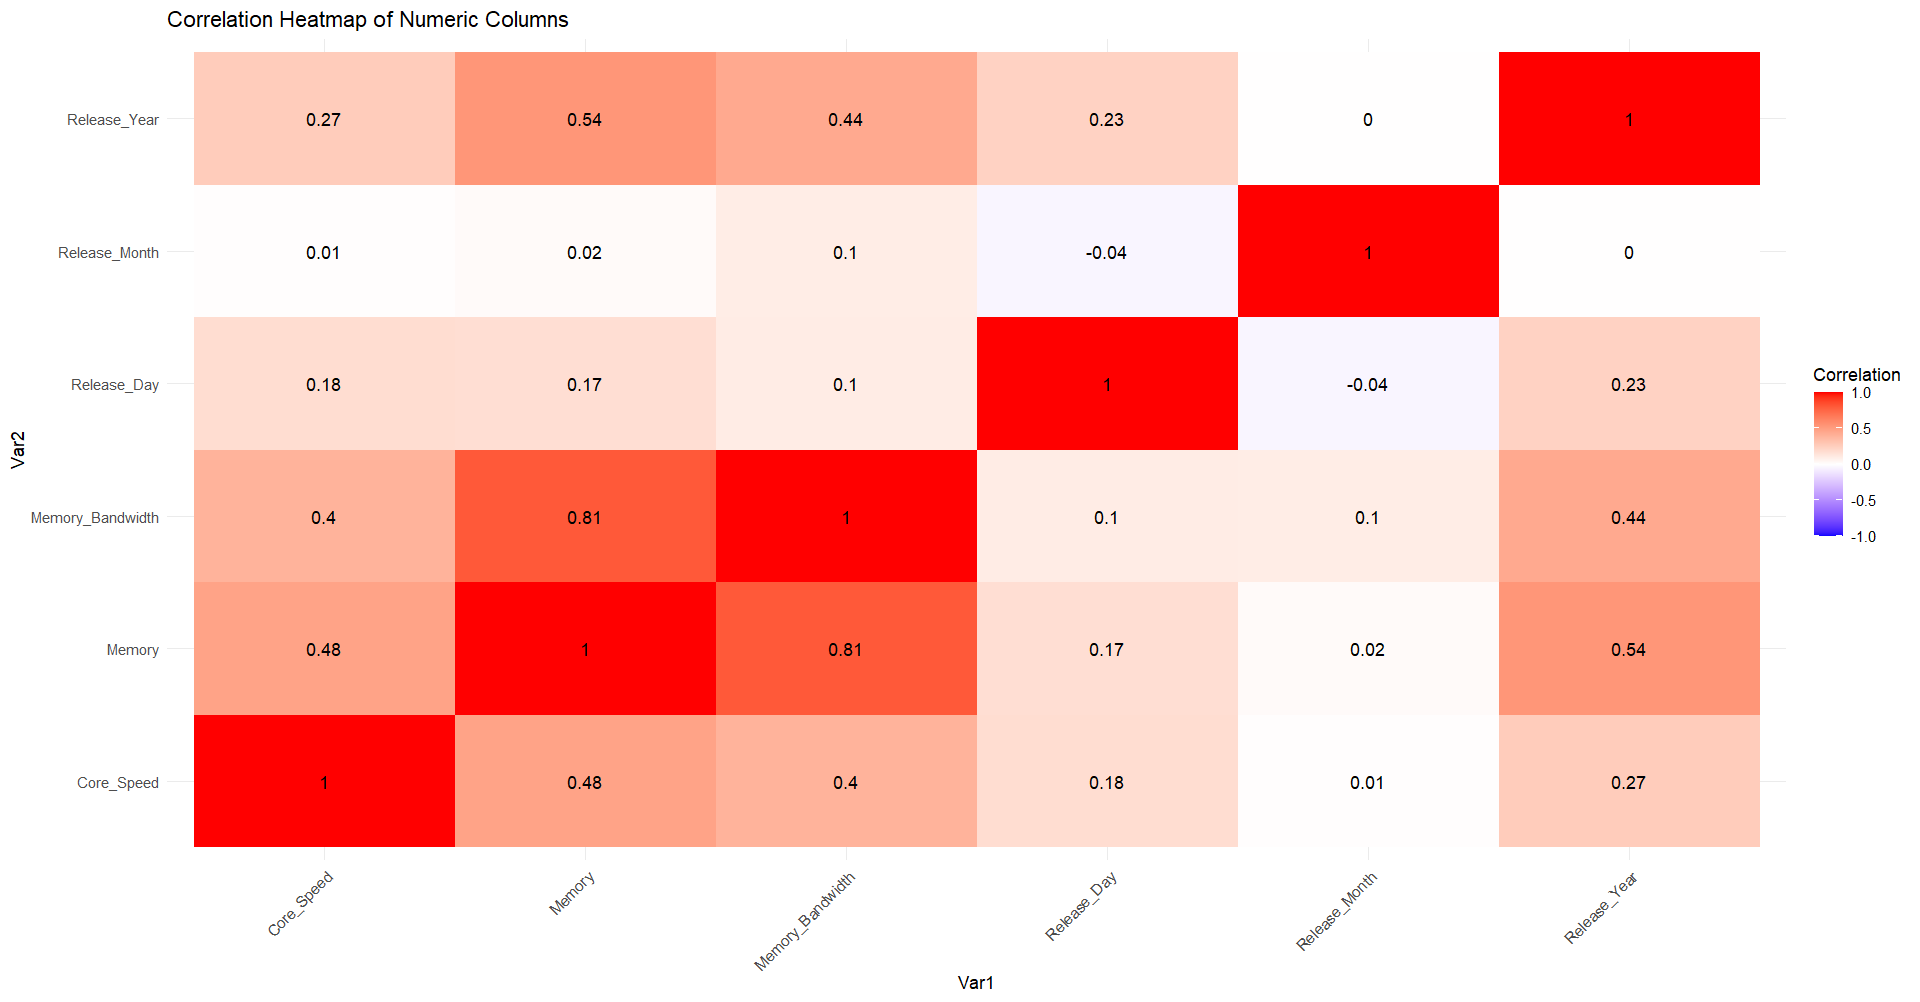
\includegraphics[width=1\linewidth]{img/GPU_cor.png}
%  \vspace{1pt}
%  \caption{Enter Caption}
%  \label{fig:enter-label}
% \end{figure}

% Nhận xét:

% \newpage
